%%%%%%%%%%%%%%%%%%%%%%%%%%%%%%%%%%%%%%%%%%%%%%%%%%%%%%%%%%%%%%%%%%%%%%%% 
%%%%%%%%%%%%%%%%%%%%%%%%%%%%%%%%%%%%%%%%%%%%%%%%%%%%%%%%%%%%%%%%%%%%%%%% 
\begin{frame}
  \frametitle{About Kokkos in Trilinos}

  \begin{itemize}
  \item \myhref{https://github.com/kokkos/kokkos}{kokkos} is originally a subpackage of \myhref{https://trilinos.org/}{trilinos} (application framework for solving problems requiring parallel large distributed linear algebra solvers).
  \item \textcolor{red}{Kokkos is the performance portable layer}, to allow running Trilinos as efficiently as possible on multiple architectures.
  \item \textbf{Kokkos can be build independently from Trilinos} and used in other applications
  \end{itemize}

  \begin{center}
    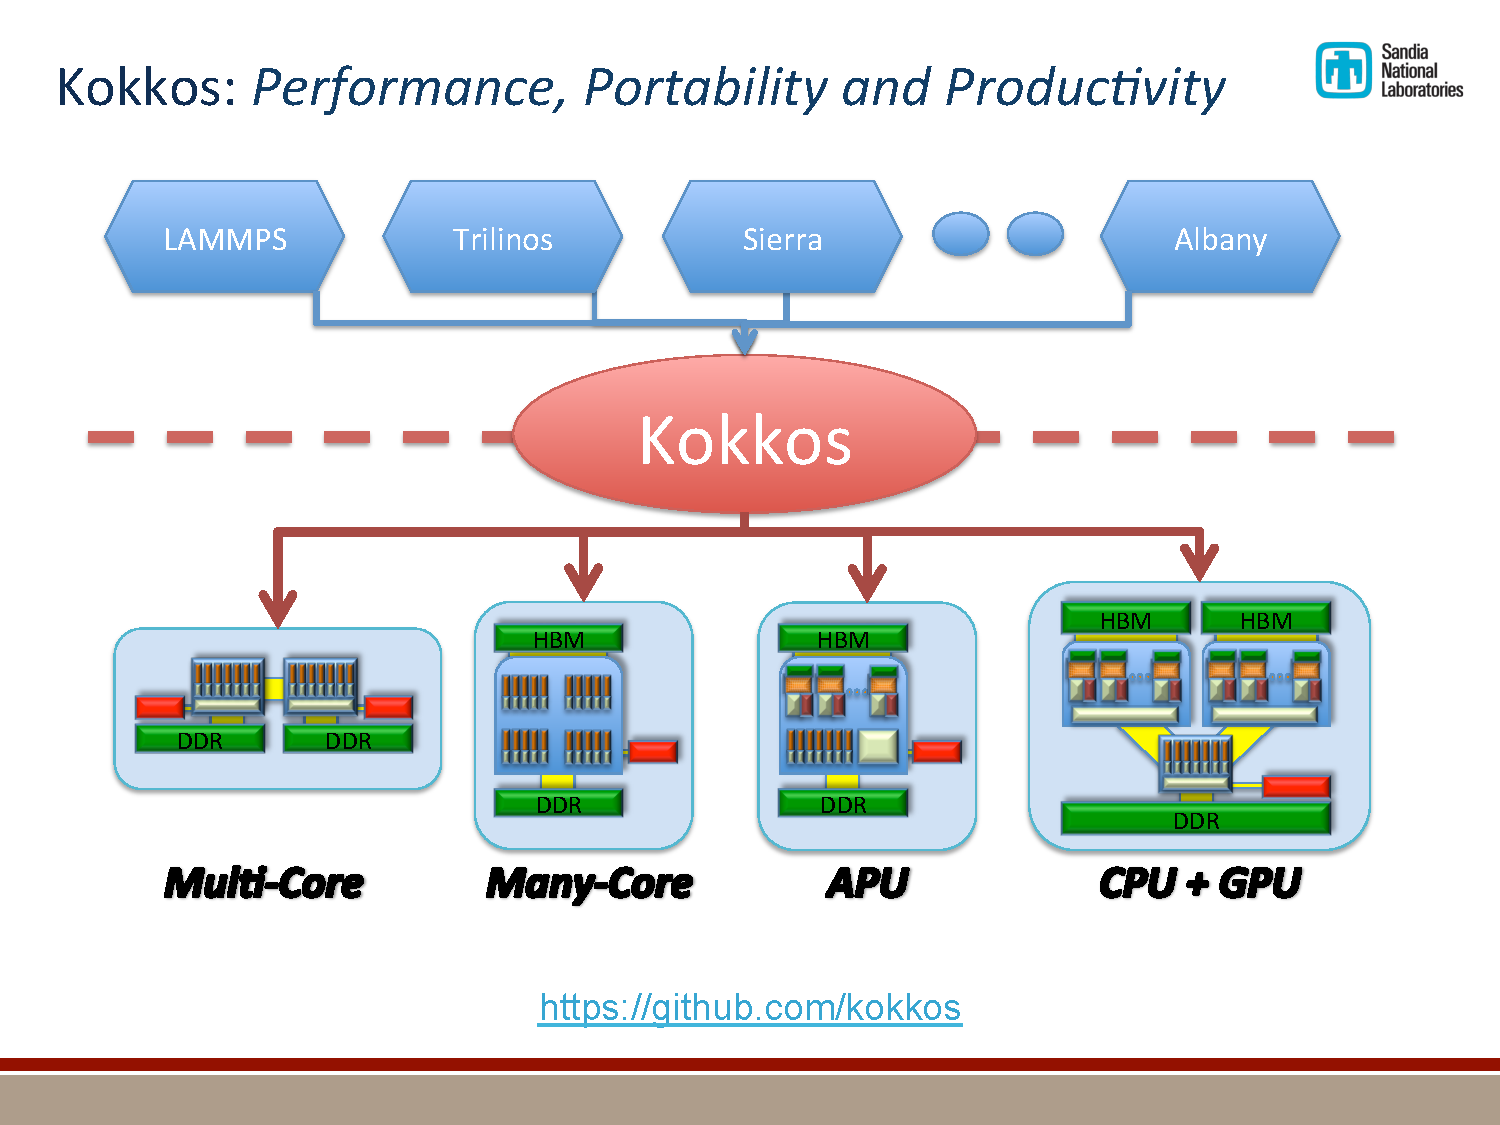
\includegraphics[width=6cm]{images/Kokkos-Multi-CoE_slide2}
  \end{center}
  
\end{frame}

%%%%%%%%%%%%%%%%%%%%%%%%%%%%%%%%%%%%%%%%%%%%%%%%%%%%%%%%%%%%%%%%%%%%%%%% 
%%%%%%%%%%%%%%%%%%%%%%%%%%%%%%%%%%%%%%%%%%%%%%%%%%%%%%%%%%%%%%%%%%%%%%%% 
\begin{frame}
  \frametitle{About Kokkos in Trilinos}

  \begin{itemize}
  \item \textcolor{red}{\textbf{Don't do the following on \texttt{ouessant}, your home is too small}}, just keep the spirit to try on your own machine
  \item \textbf{Build a minimal featured Trilinos with Kokkos for GPU activated} : \textcolor{red}{Tpetra + kokkos + Cuda}
    \begin{enumerate}
    \item \textbf{Example config plateform:} Ubuntu 16.04 + openmpi + cuda 8.0\\
      compiler is gcc 5.4.0
    \item \textbf{Get Trilinos sources:}\\
      \texttt{git clone https://github.com/trilinos/Trilinos.git;} \texttt{cd Trilinos; git checkout develop}
    \item \textbf{CMake configuration script:} Use the provided configuration file \texttt{configure\_tpetra\_kokkos\_cuda\_nvcc\_wrapper.sh} located in the provided archive (\texttt{doc/trilinos})\\
      this script needs slights changes (var \texttt{OMPI\_CXX} and install prefix)\\
      this script must be run in a build directory (not directly in trilinos sources).\\
      this config will build kokkos with unit tests and examples.
    \item \textbf{Build:} \texttt{make -j; make install}
    \item \textbf{Build a sample project.}
    \end{enumerate}
  \end{itemize}

\end{frame}

%%%%%%%%%%%%%%%%%%%%%%%%%%%%%%%%%%%%%%%%%%%%%%%%%%%%%%%%%%%%%%%%%%%%%%%% 
%%%%%%%%%%%%%%%%%%%%%%%%%%%%%%%%%%%%%%%%%%%%%%%%%%%%%%%%%%%%%%%%%%%%%%%% 
\begin{frame}
  \frametitle{Trilinos/Tpetra example project}

  \begin{itemize}
  \item Directory \texttt{doc/trilinos/tpetra\_example} contains a minimal example application for trilinos/tpetra. You just need to set env variable \texttt{TRILINOS\_PATH} to install directory.
  \end{itemize}
  
\end{frame}
